\subsection{\href{http://www.nanocut.com/}{Nanocut 2.0}}
   \hypertarget{subsec:nanocut}
   Para la firma Nanocut de Moldavia, a mitad del 2019,  se desarrolló un controlador de motor \textit{permanent
   magnet synchronous motor} (PMSM) utilizando una placa de desarrollo de Texas Instruments con un microcontrolador de tiempo real de la linea C2000 sobre la cual se desarrollaron los algoritmos de control de torque, velocidad y posición a lazo cerrados utilizando un encoder óptico relativo.\\
   Se logró poner en marcha un prototipo que sera la base de hardware y firmware para un nuevo driver genérico de motores para las máquinas CNC que cuenta dicha empresa. \\
   Se utilizó un método de control vectorial FOC, y se implementaron las transformadas de Clarke/Parke y varios PID's anidados para lograr los objetivos con la máxima performance. \\
   En la figura \ref{fig:nanocut_electronica} se pueden ver las herramientas de hardware y los algoritmos implementados en funcionamiento.\\
     \begin{figure}
      \begin{center}
         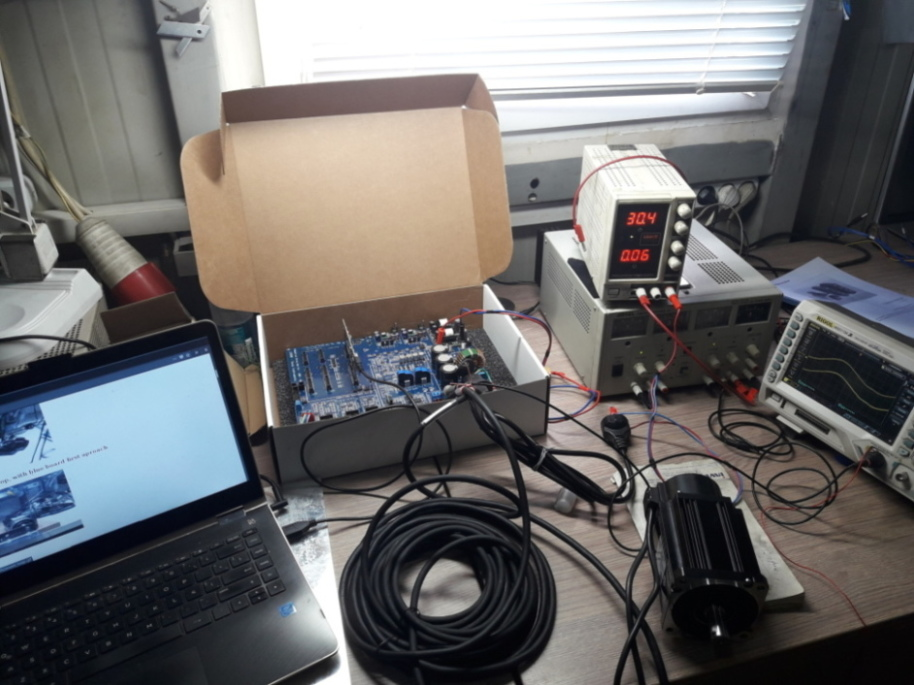
\includegraphics[width=0.3\textwidth]{nanocut1.jpg}
         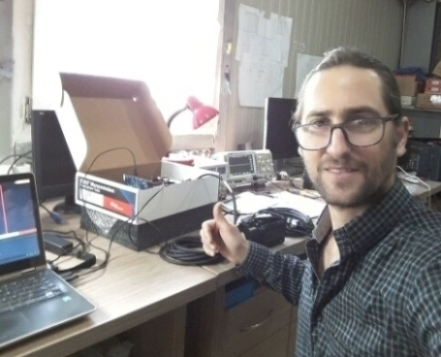
\includegraphics[width=0.3\textwidth]{nanocut2.jpg}
         
\includegraphics[width=0.3\textwidth]{nanocut3.jpg}
      \end{center}
      \caption{Herramientas de desarrollo y captura de resultados de los algoritmos para el control de un motor PMSM}
      \label{fig:nanocut_electronica}
   \end{figure}
   En la figura \ref{fig:nanocut_mecanica} se muestra el prototipo funcionando en los laboratorios de Moldavia.
  \begin{figure}
      \begin{center}
         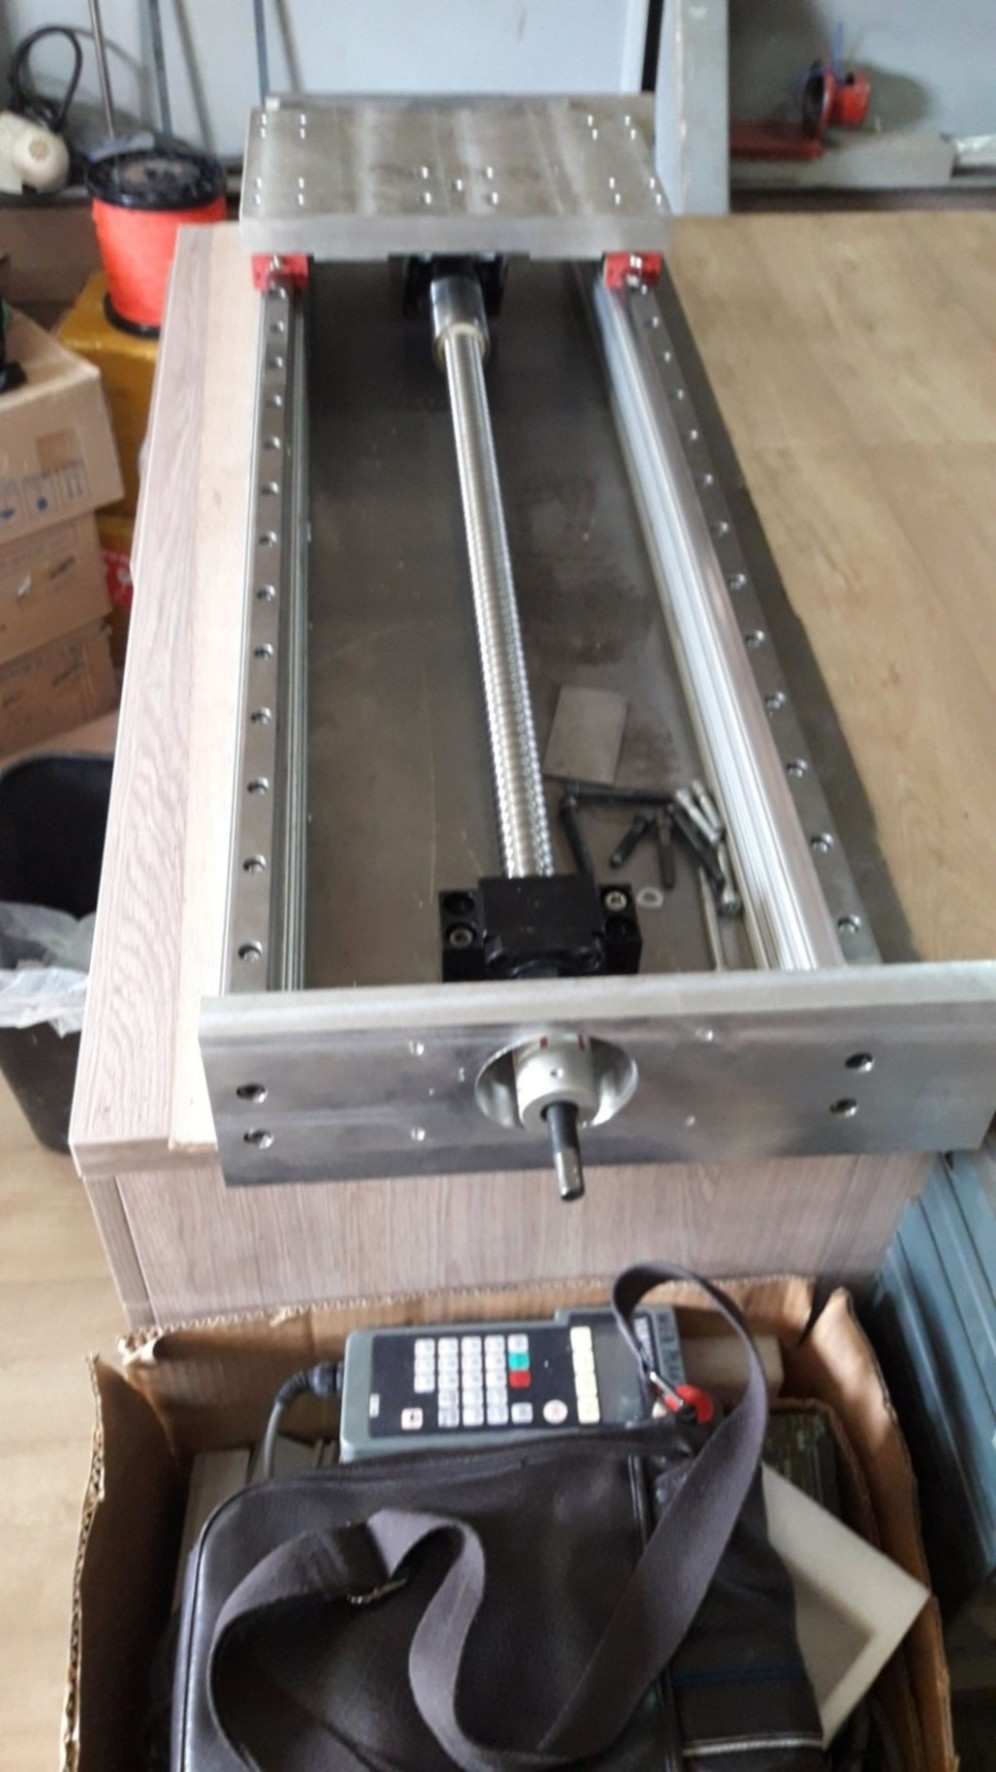
\includegraphics[width=0.3\textwidth]{nanocut4.jpg}
         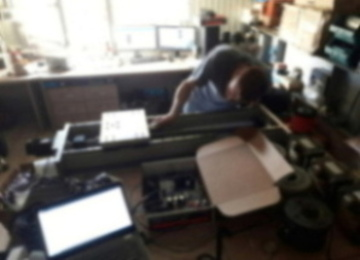
\includegraphics[width=0.3\textwidth]{nanocut5.jpg}
         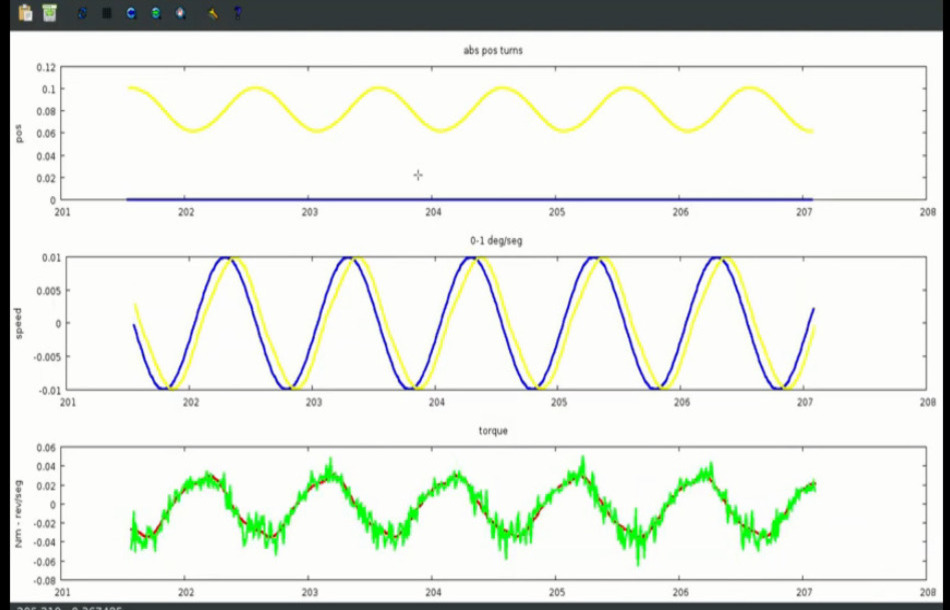
\includegraphics[width=0.3\textwidth]{nanocut6.jpg}
      \end{center}
      \caption{Prototipo mecánico para las pruebas de los algoritmos de control de torque, velocidad y posición utilizando un motor PMSM}
      \label{fig:nanocut_mecanica}
   \end{figure}

\subsection{\href{http://www.nanocut.com/}{Nanocut 3.0}}
   \hypertarget{subsec:nanocut}
   Para la firma Nanocut de Moldavia, a principio del 2020, se trabajo en el diseño de una placa de control de servo motores.
   Se diseñaron los esquemáticos, el ruteo y los modelos 3d de algunas de sus partes y del gabinete. 
   Se utilizo para el trabajo el CAD Kicad 5.0 y se utilizo un stack de 6 layers, pistas de 6mils/6mils y vías de 0.3mm para soportar el exigente encapsulado BGA de 337 patas que se utilizo.

   En total el trabajo contó con 
   \begin{itemize}
      \item{2253 pads}
      \item{728 vías}
      \item{8531 segmentos de pistas}
      \item{552 nets}
      \item{19 páginas de esquemáticos}
   \end{itemize}

   Este es el link del repositorio publico del proyecto en Github \href \linkgithubnanocutpcb {Github Nanocut}
   Se doto a la placa de circuito impreso de las siguientes capacidades técnicas:
   \begin{itemize}
      \item{procesador de triple core de tiempo real de 32b y 200mhzr}
      \item{Entrada para encoder incremental diferencial aislado x2}
      \item{Entrada para encoder absoluto diferencial aislado x2}
      \item{Entrada para pulso y dirección diferencial aislado x2}
      \item{Conexión RS485 aislado x1}
      \item{Conexión CAN aislado x1}
      \item{Conexión Ethercat esclavo x1}
      \item{Conexión Ethernet}
      \item{Medición aislada de corriente utilizando amperímetros de efecto Hall LEM's x6}
      \item{Medición aislada de voltage de linea x2}
      \item{Salida aislada de PWM para IGBT x12}
      \item{Entrada aislada para alarma x2}
      \item{Salida aislada para comandar el freno mecánico x2}
      \item{Entrada aislada para medicino de RPM's de ventilador x2}
      \item{Entrada de comunicación Sigma-Delta para medición de corriente y voltage x8}
      \item{Entrada aislada para medición de temperatura utilizando sensores NTC x4}
      \item{Comunicación 1-Wire aislada x1}
      \item{Canal SPI para conectar un LCD con touch panel del tipo EVE para proveer de una GUI completa o bien LCD de caracteres x1}
      \item{Doble fuente de alimentación aislada}
   \end{itemize}

   Se espera que con estas características la placa pueda controlar hasta 2 servo motores simultáneamente entre otras funciones.
   En la figura \ref{fig:nanocut_3_0_1} se pueden ver algunas fotos del proceso de diseño.
  \begin{figure}
      \begin{center}
         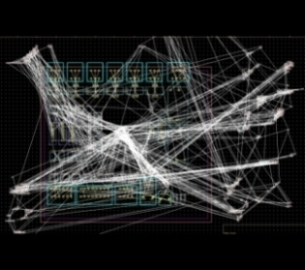
\includegraphics[width=0.3\textwidth]{nanocut_3_0_1.jpg}
         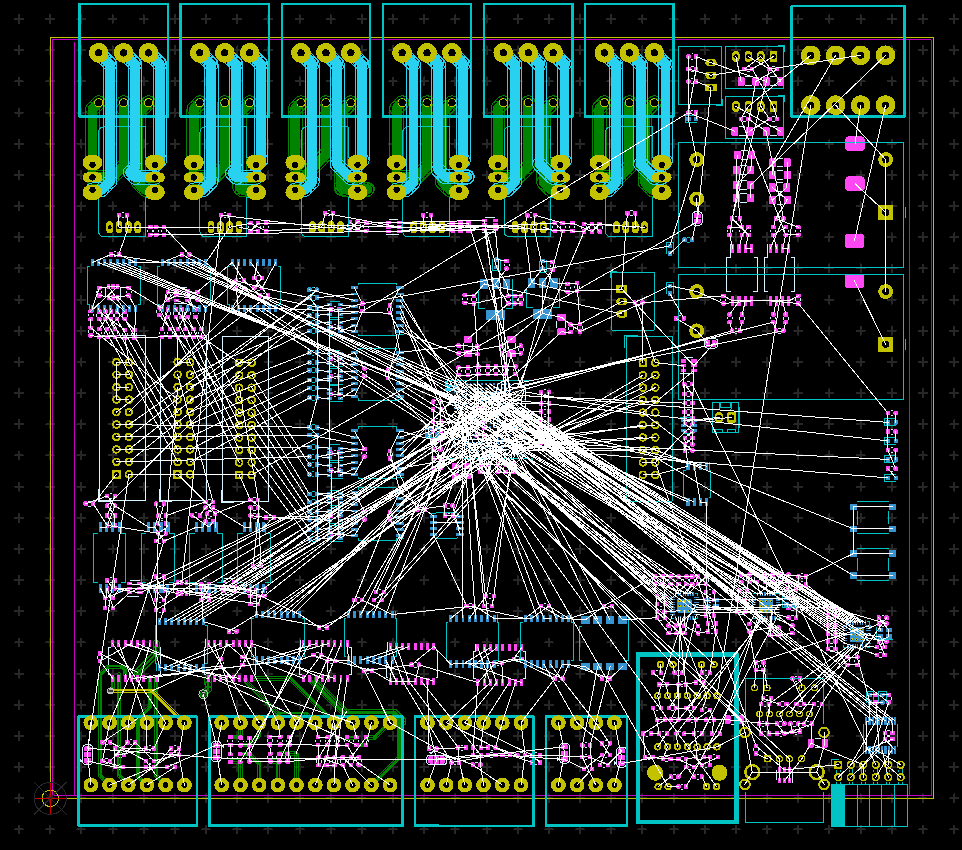
\includegraphics[width=0.3\textwidth]{nanocut_3_0_2.jpg}
         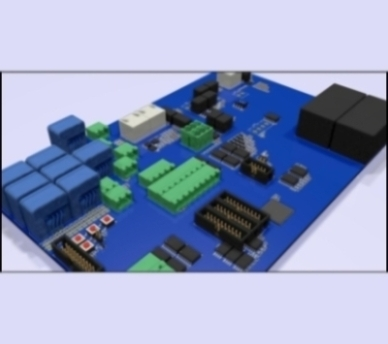
\includegraphics[width=0.3\textwidth]{nanocut_3_0_3.jpg}
      \end{center}
      \caption{Etapas del proceso de diseño de PCB para un servo drive de la empresa Nanocut}
      \label{fig:nanocut_3_0_1}
   \end{figure}

   En la figura \ref{fig:nanocut_3_0_2} se puede ver el PCB terminado y modelado en 3d con el gabinete preliminar
  \begin{figure}
      \begin{center}
         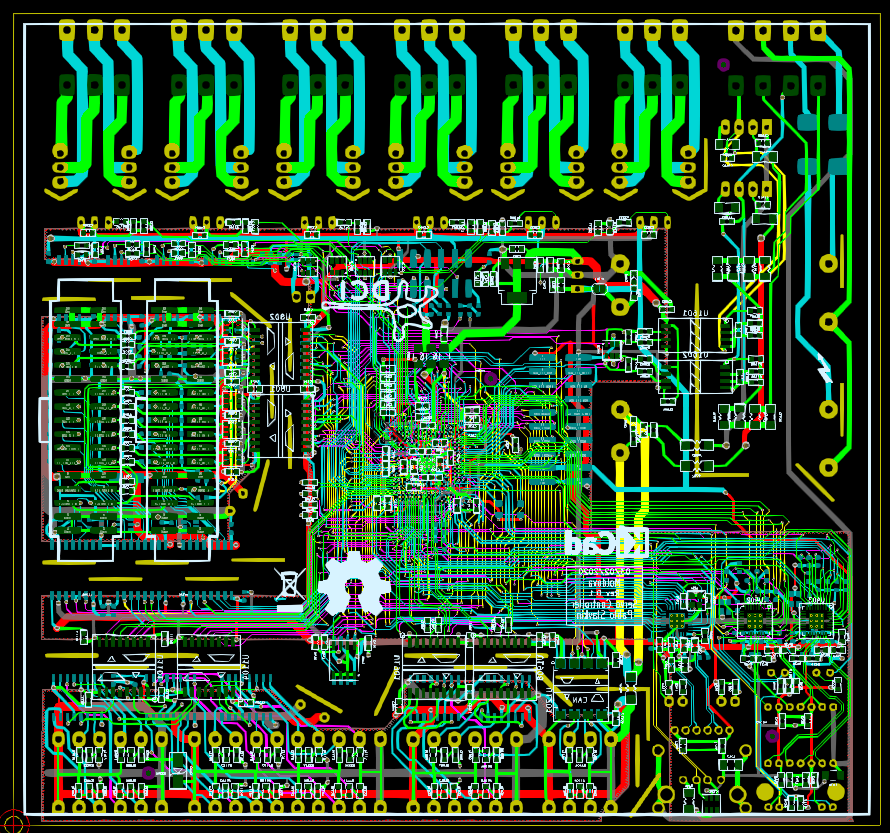
\includegraphics[width=0.3\textwidth]{nanocut_3_0_4.jpg}
         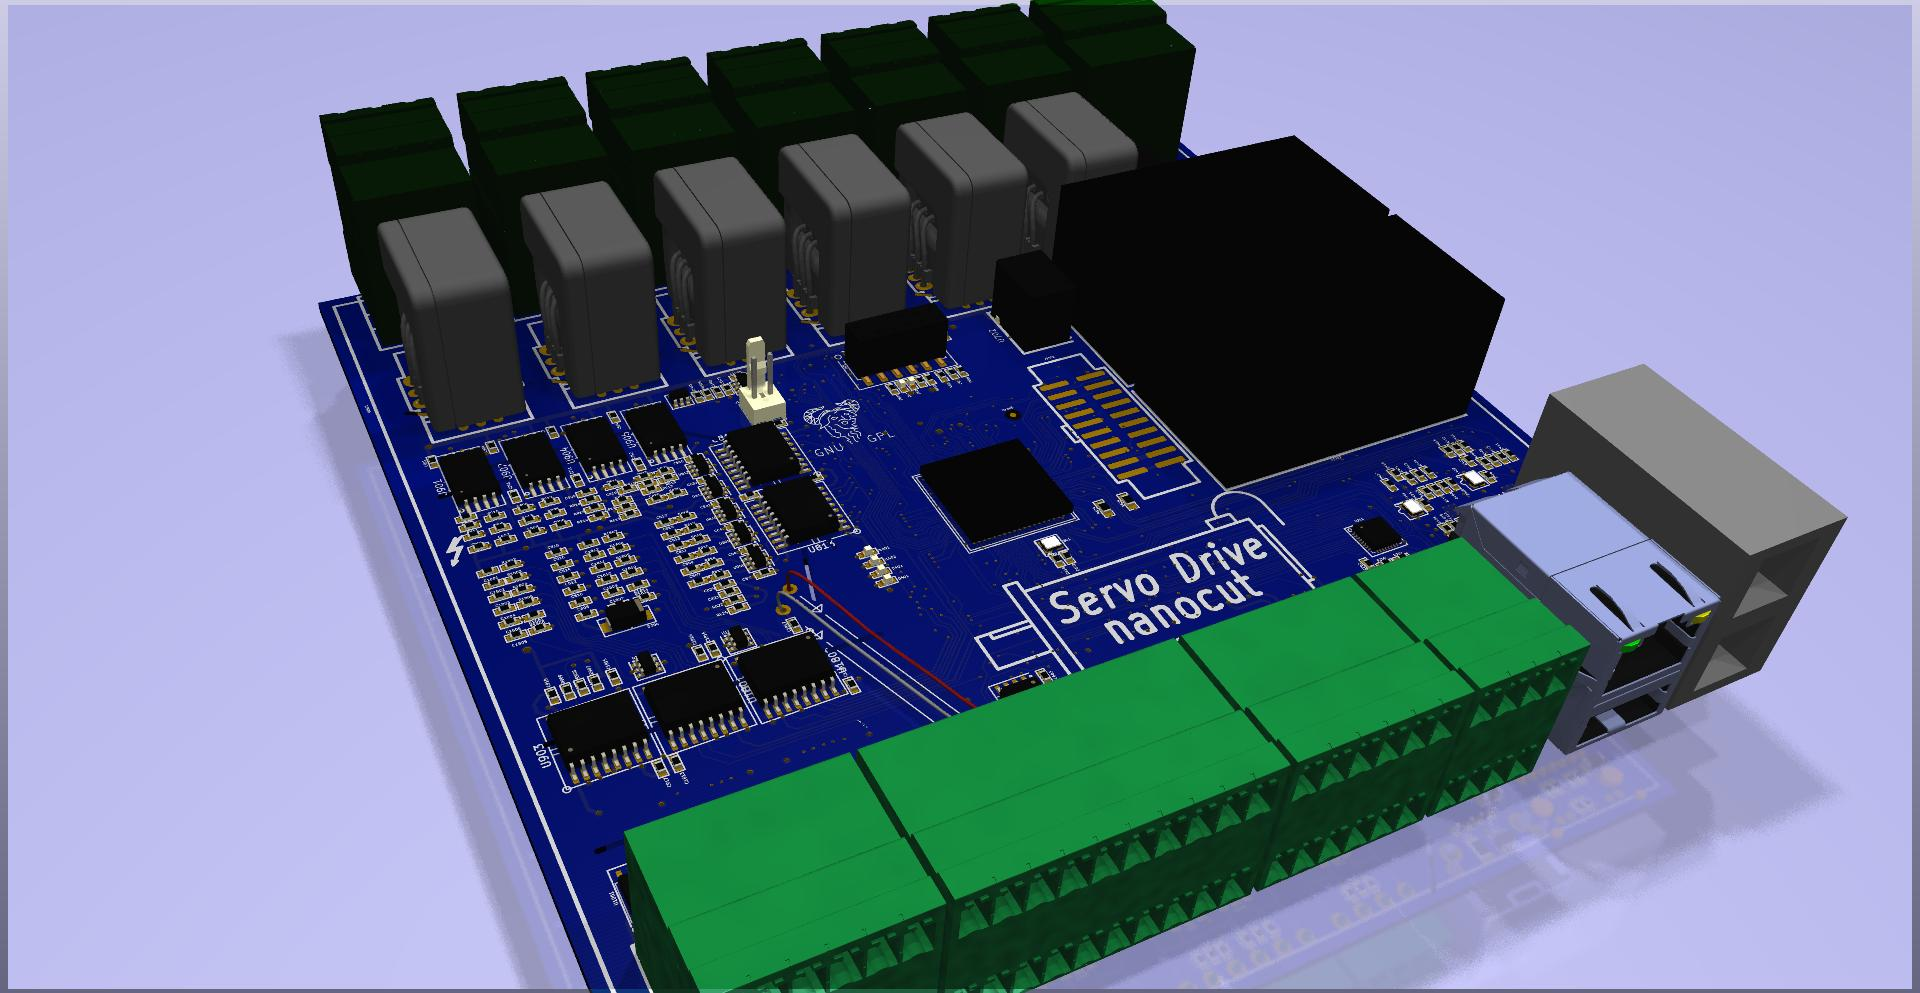
\includegraphics[width=0.3\textwidth]{nanocut_3_0_5.jpg}
         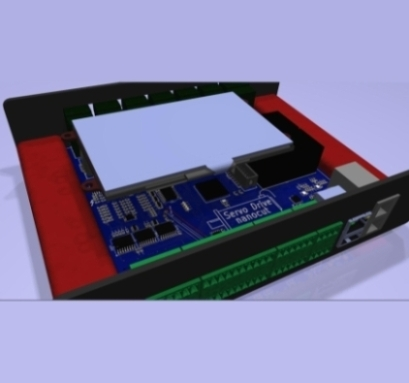
\includegraphics[width=0.3\textwidth]{nanocut_3_0_6.jpg}
      \end{center}
      \caption{Diseño de PCB completo y modelo 3D con su gabinete y LCD}
      \label{fig:nanocut_3_0_2}
   \end{figure}

